\documentclass[border=0pt]{standalone}
\usepackage{tikz}
\usetikzlibrary{calc}

\definecolor{bgtop}{HTML}{101A3A}
\definecolor{bgbot}{HTML}{060A1A}
\definecolor{floor}{HTML}{0E1733}
\definecolor{wall}{HTML}{34436E}
\definecolor{steel}{HTML}{A9BCD3}
\definecolor{ap}{HTML}{38BDF8}
\definecolor{ftm}{HTML}{F5A524}
\definecolor{rng}{HTML}{34D399}
\definecolor{pinc}{HTML}{FF4D6D}
\definecolor{gnss}{HTML}{C4B5FD}

% \satellite{x}{y}
\newcommand{\satellite}[2]{%
  \begin{scope}[shift={(#1,#2)},rotate=-20]
    \fill[steel] (-0.16,-0.12) rectangle (0.16,0.12);
    \fill[gnss!70!black,draw=gnss,line width=0.6pt] (-0.75,-0.09) rectangle (-0.22,0.09);
    \fill[gnss!70!black,draw=gnss,line width=0.6pt] (0.22,-0.09) rectangle (0.75,0.09);
    \draw[steel,line width=0.8pt] (-0.22,0) -- (-0.16,0) (0.16,0) -- (0.22,0);
    \foreach \x in {-0.62,-0.49,-0.36,0.36,0.49,0.62}{\draw[gnss!40!black,line width=0.4pt] (\x,-0.09) -- (\x,0.09);}
    \draw[steel,line width=0.8pt] (0,-0.12) -- (0,-0.24);
    \fill[steel] (0,-0.27) circle (0.05);
  \end{scope}
}

% \ap{x}{y}: ceiling access point with Wi-Fi arcs
\newcommand{\ap}[2]{%
  \begin{scope}[shift={(#1,#2)}]
    \fill[ap,opacity=0.14] (0,0) circle (0.62);
    \fill[floor,draw=ap,line width=1.3pt] (0,0) circle (0.24);
    \fill[ap] (0,0) circle (0.07);
    \foreach \r in {0.36,0.48}{\draw[ap,line width=1pt,line cap=round] (45:\r) arc[start angle=45,end angle=135,radius=\r];}
  \end{scope}
}

\begin{document}
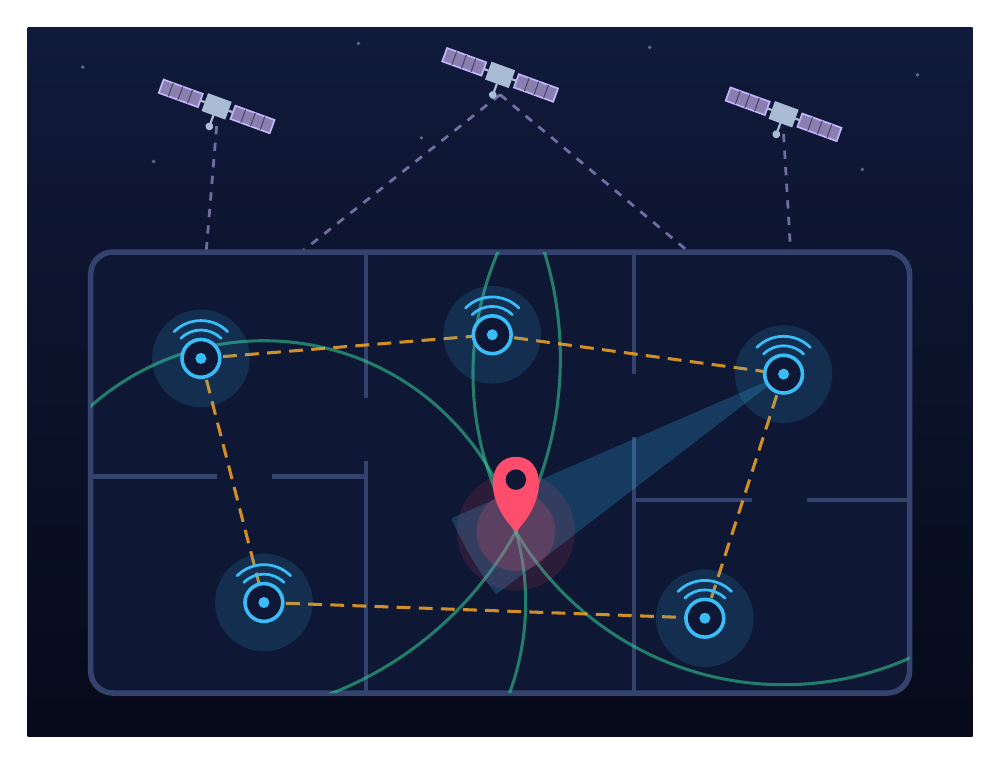
\begin{tikzpicture}
  \useasboundingbox (0,0) rectangle (12,9);
  \clip (0,0) rectangle (12,9);
  \shade[top color=bgtop,bottom color=bgbot] (0,0) rectangle (12,9);
  \foreach \x/\y in {0.7/8.5,4.2/8.8,7.9/8.75,11.3/8.4,1.6/7.3,10.6/7.2,5.0/7.6}{\fill[white,opacity=0.35] (\x,\y) circle (0.025);}

  % GNSS signals to window-side anchor APs
  \draw[gnss,opacity=0.55,line width=1pt,dash pattern=on 3pt off 3pt] (2.4,7.75) -- (2.2,5.35);
  \draw[gnss,opacity=0.55,line width=1pt,dash pattern=on 3pt off 3pt] (6.0,8.15) -- (2.4,5.30);
  \draw[gnss,opacity=0.55,line width=1pt,dash pattern=on 3pt off 3pt] (6.0,8.15) -- (9.6,5.15);
  \draw[gnss,opacity=0.55,line width=1pt,dash pattern=on 3pt off 3pt] (9.6,7.65) -- (9.75,5.15);
  \satellite{2.4}{8.0}
  \satellite{6.0}{8.4}
  \satellite{9.6}{7.9}

  % floor plan
  \fill[floor,rounded corners=8pt] (0.8,0.55) rectangle (11.2,6.15);
  \draw[wall,line width=2pt,rounded corners=8pt] (0.8,0.55) rectangle (11.2,6.15);
  \begin{scope}[wall,line width=1.6pt]
    \draw (4.3,6.15) -- (4.3,4.3);  \draw (4.3,3.5) -- (4.3,0.55);
    \draw (7.7,6.15) -- (7.7,4.6);  \draw (7.7,3.8) -- (7.7,0.55);
    \draw (0.8,3.3) -- (2.4,3.3);   \draw (3.1,3.3) -- (4.3,3.3);
    \draw (7.7,3.0) -- (9.2,3.0);   \draw (9.9,3.0) -- (11.2,3.0);
  \end{scope}

  \begin{scope}
    \clip[rounded corners=8pt] (0.8,0.55) rectangle (11.2,6.15);
    % range circles from three APs converging on the device
    \draw[rng,opacity=0.55,line width=1.1pt] (2.2,4.8) circle ({sqrt((6.2-2.2)^2+(2.6-4.8)^2)});
    \draw[rng,opacity=0.55,line width=1.1pt] (9.6,4.6) circle ({sqrt((6.2-9.6)^2+(2.6-4.6)^2)});
    \draw[rng,opacity=0.55,line width=1.1pt] (3.0,1.7) circle ({sqrt((6.2-3.0)^2+(2.6-1.7)^2)});
    % angle-of-arrival wedge from an AP toward the device
    \pgfmathsetmacro{\aoa}{atan2(2.6-4.6,6.2-9.6)}
    \fill[ap,opacity=0.22] (9.6,4.6) -- ++(\aoa-7:4.6) arc[start angle=\aoa-7,end angle=\aoa+7,radius=4.6] -- cycle;
  \end{scope}

  % FTM ranging between APs
  \foreach \a/\b in {{2.2,4.8}/{5.9,5.1},{5.9,5.1}/{9.6,4.6},{2.2,4.8}/{3.0,1.7},{9.6,4.6}/{8.6,1.5},{3.0,1.7}/{8.6,1.5}}{
    \draw[ftm,opacity=0.85,line width=1.1pt,dash pattern=on 5pt off 3pt] (\a) -- (\b);
  }

  % access points
  \ap{2.2}{4.8}
  \ap{5.9}{5.1}
  \ap{9.6}{4.6}
  \ap{3.0}{1.7}
  \ap{8.6}{1.5}

  % located device with pin
  \begin{scope}[shift={(6.2,2.6)}]
    \foreach \r/\o in {0.75/0.12,0.5/0.2}{\fill[pinc,opacity=\o] (0,0) circle (\r);}
    \fill[pinc] (0,0) .. controls (-0.42,0.42) and (-0.36,0.95) .. (0,0.95) .. controls (0.36,0.95) and (0.42,0.42) .. (0,0);
    \fill[floor] (0,0.66) circle (0.13);
  \end{scope}
\end{tikzpicture}
\end{document}
